% 第1章第4节：非线性轨道的长期行为（极限集合与吸引子；参数变化与分岔；敏感依赖与有限精度）。

\section{非线性轨道的长期行为}
\label{sec:dds-nonlinear-long-term}

上一节的判据围绕一个平衡点展开：轨道会不会回到它。非线性系统的长期行为丰富得多。轨道可能被一条周期轨道吸引而永不停下，不同初值可能去往不同的终点，参数稍作改变，终点的数目和稳定性也可能突然改变；还有些轨道始终有界，却既不收敛也不周期，近邻的两条轨道以指数速度分开。本节保持同一个问题——“轨道最终到哪里，结论如何随参数和初值改变”——依次讨论描述终点的极限集合、参数变化引起的分岔，以及敏感依赖对有限精度计算的影响。

\subsection{极限集合与吸引子}
\label{sec:dds-limit-sets}

\paragraph{有界而不收敛的轨道}
$r=3.2$时，Logistic映射的轨道趋向周期二轨道$\{x_-,x_+\}$。序列$x_n$本身没有极限，它的偶数项和奇数项却分别收敛到$x_-$与$x_+$（或者相反）。要描述这样的长期行为，“极限”需要从一个点推广为一个集合：收集轨道在越来越晚的时刻反复靠近的所有点。

\begin{definition}[$\omega$极限集]
\label{def:dds-omega-limit}
设$X\subseteq\mathbb R^d$，$F:X\to X$，$\bm x_0\in X$，$\bm x_n=F^n(\bm x_0)$。称
\[
  \omega(\bm x_0)=\bigl\{\bm z\in\mathbb R^d:\text{存在}\ n_j\to\infty\ \text{使}\ \bm x_{n_j}\to\bm z\bigr\}
\]
为$\bm x_0$的\term{$\omega$极限集}（$\omega$-limit set），即轨道全部子列极限组成的集合。
\end{definition}

等价地，$\omega(\bm x_0)=\bigcap_{N\geq0}\overline{\{\bm x_n:n\geq N\}}$：一个点属于极限集，当且仅当轨道无论多晚都还会回到它的任意邻域。几个例子显示了极限集的不同形态。轨道收敛到$\bm x_*$时，$\omega(\bm x_0)=\{\bm x_*\}$。上面的Logistic轨道有$\omega(x_0)=\{x_-,x_+\}$。$x_{n+1}=x_n+1$的轨道趋于无穷，没有任何收敛子列，$\omega(x_0)=\varnothing$。

极限集也可以是一整条曲线。把单位圆上的点记为角度$\theta\in[0,1)$（以整圈为单位），考察转动$\theta_{n+1}=\theta_n+\alpha\pmod1$。若$\alpha=p/q$是有理数，每条轨道都是周期$q$的轨道。若$\alpha$是无理数，轨道在圆上稠密，从而$\omega(\theta_0)$是整个圆。证明只用抽屉原理：$\alpha$无理时各点$\theta_n=\theta_0+n\alpha\pmod1$两两不同；任取正整数$N$，前$N+1$个点中必有两个相距小于$1/N$，设为$\theta_i,\theta_j$（$i<j$），则转动$k=j-i$步相当于沿圆周移动一个非零的距离$\beta<1/N$。从任意$\theta_m$开始，每$k$步前进$\beta$，所以轨道的后段以小于$1/N$的间隔走遍整个圆，圆上每个长度为$1/N$的弧都会被无限次访问。$N$任意，即得结论。这条轨道既不收敛也不周期，却在长期中均匀地扫过一个集合。

\paragraph{极限集合的基本性质}
极限集在什么条件下可以作为“轨道的终点”使用？至少需要它非空，并且轨道真的趋近它。下面的定理说明，轨道停留在一个紧集中时这两点都成立，而且极限集本身是不变集。

\begin{theorem}[$\omega$极限集的性质]
\label{thm:dds-omega-limit-properties}
设$X\subseteq\mathbb R^d$为闭集，$F:X\to X$连续，$\bm x_0\in X$的轨道包含在某个紧集$K\subseteq X$中。则$\omega(\bm x_0)$非空、紧，满足$F(\omega(\bm x_0))=\omega(\bm x_0)$，并且
\[
  \operatorname{dist}\bigl(\bm x_n,\omega(\bm x_0)\bigr)\to0\qquad(n\to\infty).
\]
\end{theorem}

\begin{proof}
记$\omega=\omega(\bm x_0)$。由Bolzano--Weierstrass定理，$K$中的序列$(\bm x_n)$有收敛子列，故$\omega\neq\varnothing$，且$\omega\subseteq K$。$\omega$是闭集$\overline{\{\bm x_n:n\geq N\}}$的交，因而闭；作为紧集$K$的闭子集，它是紧集。

正向不变：若$\bm x_{n_j}\to\bm z$，由连续性$\bm x_{n_j+1}=F(\bm x_{n_j})\to F(\bm z)$，所以$F(\bm z)\in\omega$。反向包含：设$\bm x_{n_j}\to\bm z$，序列$(\bm x_{n_j-1})$在$K$中，有子列收敛到某个$\bm w\in\omega$，沿这一子列$F(\bm x_{n_j-1})=\bm x_{n_j}\to\bm z$，故$F(\bm w)=\bm z$。于是$\omega\subseteq F(\omega)$。

趋近：若结论不成立，存在$\varepsilon>0$与$n_j\to\infty$使$\operatorname{dist}(\bm x_{n_j},\omega)\geq\varepsilon$。在$K$中取其收敛子列，极限属于$\omega$，与距离至少为$\varepsilon$矛盾。
\end{proof}

紧性不可省略：$x_{n+1}=x_n+1$满足其余所有条件，极限集却是空集。有了这个定理，第~\ref{sec:dds-lyapunov}小节非严格下降的结论可以说得更紧凑。在定理~\ref{thm:dds-lasalle}的条件下，$\omega(\bm x_0)$是不变集，并且其中每一点的整条正向轨道都留在$E$中；所以$\omega(\bm x_0)$包含于$E$的最大不变子集$M$，轨道趋近$M$。这就是离散时间的\term{LaSalle不变性原理}（LaSalle invariance principle）。

\paragraph{吸引子与吸引域}
有了极限集，就可以谈论“一群初值共同的终点”。文献中吸引子的定义并不统一，有的还要求稳定性或不可再分；本章采用下面的版本，并在使用时注明。

\begin{definition}[吸引子与吸引域]
\label{def:dds-attractor}
设$F:X\to X$连续，$A\subseteq X$为非空紧集且$F(A)=A$。若存在包含$A$的开集$W$，使每个$\bm x_0\in W$满足$\operatorname{dist}(F^n(\bm x_0),A)\to0$，称$A$为\term{吸引子}（attractor）。集合
\[
  \mathcal B(A)=\{\bm x_0\in X:\operatorname{dist}(F^n(\bm x_0),A)\to0\}
\]
称为$A$的\term{吸引域}（basin of attraction）。
\end{definition}

渐近稳定的平衡点$\{\bm x_*\}$与稳定的周期轨道都是吸引子。吸引域通常比证明得到的子水平集大得多（图~\ref{fig:dds-basin-estimate}），但它有一个可以直接证明的性质：若$\bm x_*$渐近稳定、$F$在$X=\mathbb R^d$上连续，则$\mathcal B(\{\bm x_*\})$是开集。事实上，取吸引半径$r$，若$\bm x_0\in\mathcal B$，则某个$F^m(\bm x_0)$落在开球$B_r(\bm x_*)$中；$F^m$连续，所以$\bm x_0$的一个邻域也被$F^m$送进$B_r(\bm x_*)$，这个邻域中的每一点随后都收敛到$\bm x_*$。

同一个系统可以有几个吸引子，它们的吸引域把空间分成几块。图~\ref{fig:dds-newton-basins}画出用牛顿法求$z^3=1$的复根时的情形。迭代$N(z)=z-(z^3-1)/(3z^2)=(2z^3+1)/(3z^2)$以三个立方根$1,\mathrm e^{\pm2\pi\mathrm i/3}$为平衡点。由$N'(z)=2(z^3-1)/(3z^3)$，三个根处$N'=0$，线性化给出极强的局部吸引，靠近根之后误差大致每步平方一次。可是远离根时，初值去往哪个根并不显然：图中按60步后到达的根给每个初值着色，三块颜色在交界处以越来越细的尺度反复交错。

\begin{figure}[htbp]
  \centering
  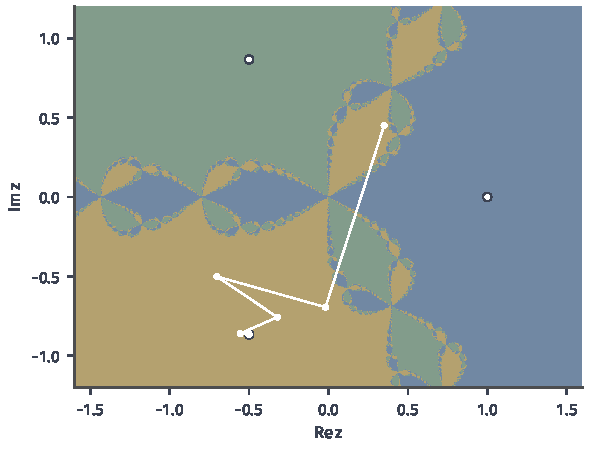
\includegraphics[width=100mm]{figures/03-optimization-evolution-and-signals/02-processes-and-trajectory-evolution/matplotlib/dds-newton-basins/figure.pdf}
  \caption{牛顿法求$z^3=1$的三个吸引域。复平面$[-1.6,1.6]\times[-1.2,1.2]$上$900\times675$个初值各迭代$N(z)=(2z^3+1)/(3z^2)$六十步，按到达的根着色：蓝色趋于$1$，绿色趋于$\mathrm e^{2\pi\mathrm i/3}$，黄色趋于$\mathrm e^{-2\pi\mathrm i/3}$；白圈为三个根。白色折线是从$0.35+0.45\mathrm i$出发的一条轨道，它先跳过原点附近，最后落入左下方的根。}
  \label{fig:dds-newton-basins}
\end{figure}

这张图同时说明了数值图像的边界。每个像素只代表一个初值的有限步计算，着色依赖迭代步数和判定容差；它提示吸引域的边界非常复杂，却不能证明边界的结构。复动力系统的理论确实证明了，这三个吸引域有共同的边界，边界上任一点附近三种颜色都会出现，但这一结论需要专门的工具，本章不证。读图时应把它当作观察，而不是定理。

一维的Logistic映射也有类似的问题，只是简单得多。$r=3.2$时，周期二轨道吸引了$(0,1)$中除可数个点以外的全部初值；这一结论需要一维映射的专门理论，这里只说明例外点为何至多可数。例外的是最终恰好落在不稳定平衡点$0$或$x_r=0.6875$上的点，例如$x_0=0.3125$满足$F(0.3125)=0.6875$。每个点在$F$下至多有两个前像，所以这些例外点可以按“几步之后落到平衡点”逐层列出，组成一个可数集。

\subsection{参数变化与分岔}
\label{sec:dds-bifurcation}

\paragraph{沿参数跟踪平衡点}
模型几乎总含参数：Logistic映射的$r$，梯度下降的步长，动量迭代的$\beta$。参数连续变化时，平衡点会不会也连续变化，稳定性会不会保持？考察一族一维映射$F_\mu(x)$，$\mu$为实参数，平衡点满足$G(x,\mu)=F_\mu(x)-x=0$。若$(x_*,\mu_0)$是一个平衡点，$F$连续可微，且
\[
  \partial_xG(x_*,\mu_0)=F_{\mu_0}'(x_*)-1\neq0,
\]
则由隐函数定理，在$\mu_0$附近存在唯一的连续可微函数$x_*(\mu)$，使$x_*(\mu)$是$F_\mu$在$x_*$附近唯一的平衡点。导数$F_\mu'(x_*(\mu))$随$\mu$连续变化，只要它不穿过$\pm1$，线性化判据给出的稳定性就保持不变。

所以平衡点的数目或稳定性只可能在$F'=1$或$F'=-1$处改变。参数经过某个值时，平衡点或周期轨道的数目、稳定性发生改变，这种现象称为\term{分岔}（bifurcation），这个参数值称为分岔点。$F'=1$时隐函数定理失效，平衡点可能成对出现或消失；$F'=-1$时平衡点本身仍可延续，但两步映射$F^2$的导数$(F')^2=1$，周期二轨道可能从这里分出。下面两个例子分别对应这两种情形。

\paragraph{鞍结分岔}
考察$F_\mu(x)=x+\mu-x^2$。平衡点方程$x=x+\mu-x^2$即$x^2=\mu$。$\mu<0$时没有平衡点，并且$x_{n+1}-x_n=\mu-x_n^2<0$，每条轨道都严格递减，最终趋于$-\infty$。$\mu>0$时有两个平衡点$\pm\sqrt\mu$。由$F_\mu'(x)=1-2x$，在$\sqrt\mu$处导数为$1-2\sqrt\mu$，当$0<\mu<1$时落在$(-1,1)$内，该点指数稳定；在$-\sqrt\mu$处导数为$1+2\sqrt\mu>1$，该点不稳定。$\mu=0$时两者合并为$x=0$，导数恰好为$1$。图~\ref{fig:dds-bifurcation-branches}(a)画出这两条分支：参数从负到正穿过$0$时，一对平衡点“凭空”出现，一稳一不稳。这种分岔称为\term{鞍结分岔}（saddle-node bifurcation）。

\begin{figure}[htbp]
  \centering
  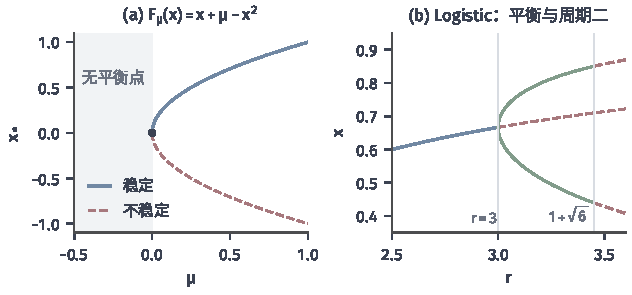
\includegraphics[width=107mm]{figures/03-optimization-evolution-and-signals/02-processes-and-trajectory-evolution/matplotlib/dds-bifurcation-branches/figure.pdf}
  \caption{两类分岔的解析分支，实线稳定、虚线不稳定。(a)$F_\mu(x)=x+\mu-x^2$的平衡点$\pm\sqrt\mu$；$\mu<0$（灰色区域）没有平衡点，$\mu=0$处两点合并，图中只画到$\mu=1$，此后$\sqrt\mu$处的导数将低于$-1$。(b)Logistic映射：平衡点$x_r=1-1/r$在$r<3$时稳定（蓝），$r>3$时失稳（红虚线）；周期二轨道$x_\pm$从$r=3$分出，在$3<r<1+\sqrt6$时稳定（绿），此后失稳。}
  \label{fig:dds-bifurcation-branches}
\end{figure}

\paragraph{倍周期分岔：Logistic映射的可解析区间}
Logistic映射在$r\in[0,4]$上把$[0,1]$映回自身，前面已经算出它的平衡点和周期二轨道，现在把这些结果按参数排起来。$0\leq r<1$时，$F_r'(0)=r<1$，原点指数稳定，$x_r=1-1/r$不在$[0,1]$中。$r$越过$1$，$x_r$进入$[0,1]$并接管稳定性：$F_r'(0)=r>1$使原点失稳，$F_r'(x_r)=2-r\in(-1,1)$对$1<r<3$成立。

$r=3$时$F_r'(x_r)=-1$。越过$3$以后，$x_r$不稳定，而式子$x_\pm=\bigl((r+1)\pm\sqrt{(r+1)(r-3)}\bigr)/(2r)$给出的周期二轨道恰好在此时出现。它的乘子是$-r^2+2r+4$：$r=3$时等于$1$，随$r$增大而减小，在$r=1+\sqrt6\approx3.449$时降到$-1$。所以$3<r<1+\sqrt6$时，周期二轨道是吸引子（图~\ref{fig:dds-bifurcation-branches}(b)）。图~\ref{fig:dds-period-two-graph}给出了几何画面：$F'(x_r)$穿过$-1$时，$F^2$在$x_r$处的斜率$(F'(x_r))^2$由小于$1$变为大于$1$，$F^2$的图像在$x_r$两侧各多穿过对角线一次，多出的两个交点就是$x_\pm$。导数穿过$-1$时，周期翻倍的轨道从原平衡点分出，原平衡点同时失稳，这称为\term{倍周期分岔}（period-doubling bifurcation）。

同样的机制出现在优化里，这时分岔参数是步长。梯度下降在最小点处的线性化导数是$1-\eta f''(x_*)$，步长增大使它穿过$-1$，迭代就从收敛变为在最小点两侧来回跳动。

\begin{example}[步长引起的倍周期分岔]
\label{ex:dds-step-size-bifurcation}
对$f(x)=x^4/4-x^2/2$作梯度下降，$F_\eta(x)=x-\eta(x^3-x)$，步长$\eta>0$。平衡点是$f$的驻点$0,\pm1$。$F_\eta'(x)=1-\eta(3x^2-1)$，在局部极大点$0$处为$1+\eta>1$，不稳定；在两个最小点处为$1-2\eta$，所以$0<\eta<1$时最小点指数稳定，$\eta=1$时导数恰为$-1$。临界步长$\eta=1$正是$2/f''(\pm1)$，与二次目标上的步长条件一致。越过$1$以后，从$x_0=1.2$出发迭代$2000$步的数值结果显示：$\eta=1.05$时轨道趋于周期二轨道$\{0.873,1.091\}$，$\eta=1.1$时为$\{0.815,1.116\}$，乘子分别约为$0.60$和$0.18$，都是稳定的；$\eta=1.2$时乘子约为$-0.68$，仍然稳定但已接近下一次翻倍。所以步长略大于临界值时，梯度下降并不发散，而是稳定地在最小点两侧跳动，目标值不再下降到最小值；这与发散是两种不同的失败方式。
\end{example}

\paragraph{分岔图：作为观察的补充}
$r>1+\sqrt6$以后，周期二轨道的乘子小于$-1$，同样的机制作用于$F^2$，分出周期四的轨道；再往后又有周期八、十六……解析计算越来越难，数值观察成了主要手段。图~\ref{fig:dds-logistic-bifurcation}上半部分对$1500$个$r$值各自丢弃前$1000$步、画出随后$400$个状态：稳定周期轨道表现为有限个点，倍周期表现为分叉；数值计算显示，翻倍发生的参数值依次约为$3$、$3.449$、$3.544$、……，间隔越来越小，在$r\approx3.5699$附近累积。此后大部分参数下点连成一片，其间又夹着若干周期窗口，最显眼的是$r\approx3.83$附近的周期三窗口。

\begin{figure*}[htbp]
  \centering
  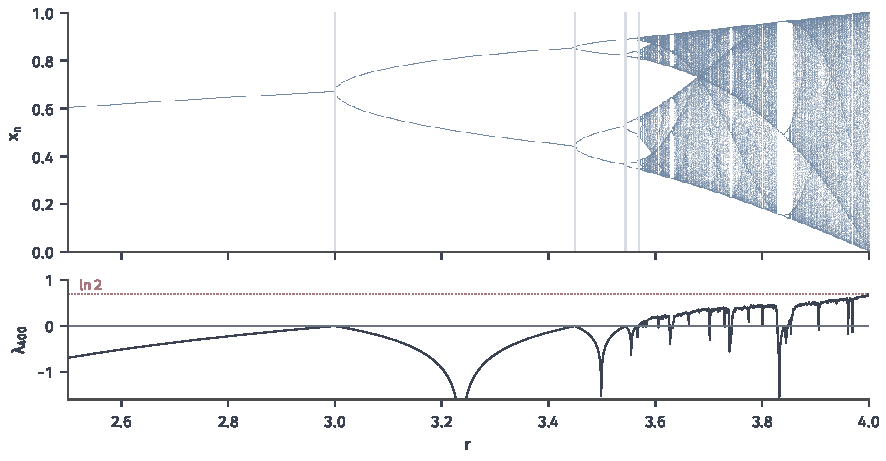
\includegraphics[width=150mm]{figures/03-optimization-evolution-and-signals/02-processes-and-trajectory-evolution/matplotlib/dds-logistic-bifurcation/figure.pdf}
  \caption{Logistic映射的分岔图与有限时间Lyapunov指数。上：对$r\in[2.5,4]$的$1500$个值，从$x_0=0.2$出发丢弃前$1000$步，画出随后$400$步的状态；竖线标出$r=3$、$1+\sqrt6$、$3.544$与累积点$3.5699$。下：同样$400$步上$\ln|F_r'(x_n)|$的平均值，零线以上表示近邻轨道平均以指数速度分离，红色点线为$\ln2$。两图都是有限步数值观察。}
  \label{fig:dds-logistic-bifurcation}
\end{figure*}

这张图容易被读得过头。点连成一片只说明有限步内轨道没有落到少数几个点上；它可能是混沌，也可能是周期很长或收敛很慢的轨道，还可能是舍入误差的产物。说某个参数下轨道“混沌”，需要证明诸如正Lyapunov指数、稠密轨道等性质，而不是看图。下一小节在$r=4$这个可以精确求解的参数上完成这样的证明。

\subsection{敏感依赖与有限精度}
\label{sec:dds-sensitivity}

\paragraph{两条近邻轨道的分离}
取$r=4$，从$x_0=0.2$和$x_0=0.2+10^{-10}$出发，用$120$位十进制精度计算两条轨道（图~\ref{fig:dds-sensitive-separation}）。前二十多步里两条轨道在图上完全重合；它们的距离却从$10^{-10}$开始，大致沿着$10^{-10}\cdot2^n$的直线增长，第$30$步超过$0.1$，此后两条轨道毫无关系。初值相差百亿分之一，三十步后的状态就无法用其中一条预测另一条，这就是\term{敏感依赖}（sensitive dependence on initial conditions）。

\begin{figure}[htbp]
  \centering
  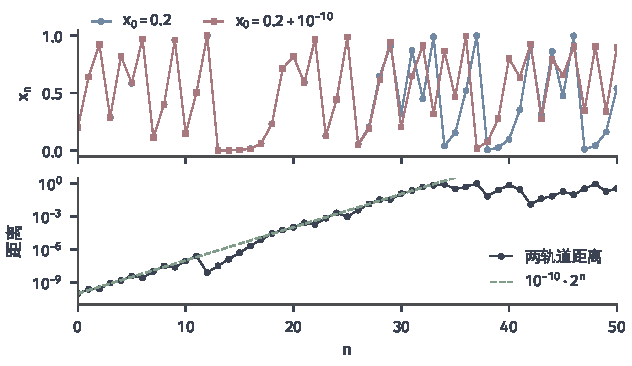
\includegraphics[width=107mm]{figures/03-optimization-evolution-and-signals/02-processes-and-trajectory-evolution/matplotlib/dds-sensitive-separation/figure.pdf}
  \caption{$r=4$时两条近邻轨道的分离。上：从$0.2$（蓝）与$0.2+10^{-10}$（红）出发的轨道，均以$120$位十进制精度计算。下：两轨道距离（对数纵轴）与参考线$10^{-10}\cdot2^n$。距离按每步约翻倍的速度增长，第$30$步超过$0.1$后在$[0,1]$的尺度上饱和；第$12$步的凹陷来自$x_{11}\approx0.504$：那里$F_4'(x)=4-8x$接近零，距离被暂时压缩，随后轨道贴近$0$，导数接近$4$，距离又迅速放大。}
  \label{fig:dds-sensitive-separation}
\end{figure}

分离速度可以用导数定量描述。设$F$可微，初值偏差$\delta$很小，则由链式法则
\[
  F^n(x_0+\delta)-F^n(x_0)\approx(F^n)'(x_0)\,\delta=\Bigl(\prod_{k=0}^{n-1}F'(x_k)\Bigr)\delta .
\]
偏差每经过一步就乘以当地的导数。把乘积取对数并平均，得到有限时间的增长率
\begin{equation}
  \lambda_n(x_0)=\frac1n\sum_{k=0}^{n-1}\ln\bigl|F'(x_k)\bigr| .
  \label{eq:dds-finite-lyapunov}
\end{equation}

\begin{definition}[Lyapunov指数]
\label{def:dds-lyapunov-exponent}
设$F$可微，且轨道$(x_k)$上$F'(x_k)\neq0$。若极限$\lambda(x_0)=\lim_{n\to\infty}\lambda_n(x_0)$存在，称为$x_0$处的\term{Lyapunov指数}（Lyapunov exponent）。
\end{definition}

指数的含义要和使用条件一起读。在稳定平衡点上，$\lambda=\ln|F'(x_*)|<0$；在乘子为$m$的稳定周期$p$轨道上，$\lambda=\frac1p\ln|m|<0$；它们都说明近邻轨道被拉拢。$\lambda>0$表示近邻轨道平均以$\mathrm e^{\lambda n}$的速度分开，但仅凭正指数不能断言轨道复杂：不稳定平衡点上也有$\lambda=\ln|F'(x_*)|>0$，而那条轨道一动不动。此外，$\lambda_n$是有限时间的量，近似式还要求偏差始终足够小；偏差长到状态空间的尺度后，线性近似就不成立了，图~\ref{fig:dds-sensitive-separation}中距离的饱和正是这个原因。图~\ref{fig:dds-logistic-bifurcation}下半部分画出了$\lambda_{400}$：周期窗口里为负，分岔点处接近$0$，连成一片的区域大多为正。

\paragraph{$r=4$时的精确解：每步翻倍的角度}
$r=4$的Logistic映射可以精确求解，敏感依赖的来源因此一目了然。令$h(\theta)=\sin^2(\pi\theta)$，则
\[
  F_4\bigl(h(\theta)\bigr)=4\sin^2(\pi\theta)\cos^2(\pi\theta)=\sin^2(2\pi\theta)=h(2\theta).
\]
所以若$x_0=h(\theta_0)$，归纳得
\begin{equation}
  x_n=\sin^2\bigl(\pi\,2^n\theta_0\bigr).
  \label{eq:dds-logistic-exact}
\end{equation}
$h$以$1$为周期，只有$\theta$的小数部分起作用；而$[0,1]$中的每个$x$都可以写成$h(\theta)$。在$\theta$坐标下，Logistic映射变成了倍角映射$\theta\mapsto2\theta\pmod1$。

把$\theta_0$写成二进制小数$0.b_1b_2b_3\ldots$，乘以$2$再取小数部分就是把各位左移一位、丢掉首位：$\theta_n=0.b_{n+1}b_{n+2}\ldots$。于是$x_n$只取决于$\theta_0$第$n+1$位以后的数字。两个初值的$\theta$若只在前$k$位一致，大约$k$步以后它们的状态就由互不相关的数字决定。初值精度每多一位二进制，可预测的步数只多一步。

指数也可以直接算出。对式$F_4\circ h=h\circ(2\,\cdot)$用链式法则$n$次，得$(F_4^n)'(h(\theta_0))\,h'(\theta_0)=2^n\,h'(\theta_n)$，其中$h'(\theta)=\pi\sin(2\pi\theta)$。在$h'(\theta_0)\neq0$（即$x_0\notin\{0,1\}$）时，
\[
  \lambda_n(x_0)=\frac1n\ln\bigl|(F_4^n)'(x_0)\bigr|=\ln2+\frac1n\ln\frac{|\sin(2\pi\theta_n)|}{|\sin(2\pi\theta_0)|}.
\]
只要轨道不越来越贴近$x=0$或$x=1$，使得$\frac1n\ln|\sin(2\pi\theta_n)|\to0$，就有$\lambda(x_0)=\ln2$；图~\ref{fig:dds-logistic-bifurcation}在$r=4$处的数值约为$0.69$，与$\ln2\approx0.693$相符。例外的轨道确实存在：$x_0=3/4$是平衡点，$F_4'(3/4)=-2$，指数恰为$\ln2$；$x_0=0$是平衡点，$F_4'(0)=4$，指数为$\ln4$；$x_0=1/2$两步后落到$0$并停住。所以“指数为$\ln2$”是对一类轨道的结论，不是对每个初值都成立。

\paragraph{有限精度：每步丢失一个比特}
敏感依赖立刻影响数值计算。双精度浮点数有$53$位二进制有效数字，单精度有$24$位。用浮点数计算$r=4$的轨道，每一步的舍入误差约为$10^{-16}$（双精度）量级，随后按每步约翻倍的速度放大。图~\ref{fig:dds-rounding-divergence}比较两种精度与$120$位十进制参考值：单精度轨道在第$23$步误差超过$0.1$，双精度在第$52$步超过$0.1$，几乎恰好是有效位数。之后算出的数仍在$[0,1]$中，看上去正常，但与从$0.2$出发的真实轨道已经没有关系。

\begin{figure}[htbp]
  \centering
  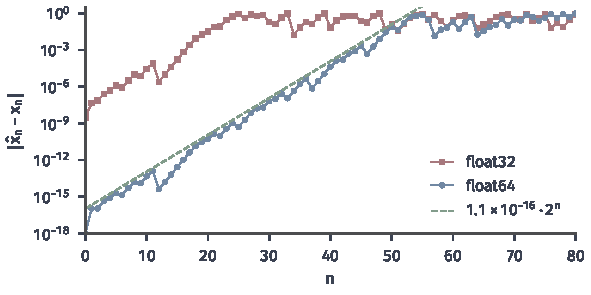
\includegraphics[width=100mm]{figures/03-optimization-evolution-and-signals/02-processes-and-trajectory-evolution/matplotlib/dds-rounding-divergence/figure.pdf}
  \caption{有限精度下$r=4$轨道的偏离。$x_0=0.2$，分别用单精度（红）与双精度（蓝）逐步计算，与$120$位十进制参考轨道比较，纵轴取对数，绿色虚线为$1.1\times10^{-16}\cdot2^n$。双精度第$0$步的误差来自$0.2$本身不能用二进制精确表示；两种精度分别在第$23$、$52$步误差超过$0.1$。}
  \label{fig:dds-rounding-divergence}
\end{figure}

这不是程序错误，而是映射本身的性质：再好的算法也不能在每步翻倍的误差面前长期保持逐点精度。提高精度只能线性地延长可预测步数，每多一位十进制数字大约多$\log_210\approx3.3$步。另一方面，逐点预测失效并不意味着一切长期陈述都失去意义。轨道在$[0,1]$中各处停留的频率、时间平均等统计性质，往往对这种误差不敏感；对某些满足专门条件的系统，还能证明计算出的轨道整段贴近另一条真实轨道。本章只建立“轨道误差”的含义，统计规律和概率描述留给第~\ref{chap:discrete-time-stochastic-processes}章。
